
%(BEGIN_QUESTION)
% Copyright 2007, Tony R. Kuphaldt, released under the Creative Commons Attribution License (v 1.0)
% This means you may do almost anything with this work of mine, so long as you give me proper credit

Når en syre tilsettes vann, dissosierer noen syremolekyler til positive hydrogenioner (H$^{+}$) og negative ioner (typen avhenger av syren). Dette øker hydrogenion-molariteten. Samtidig reduseres hydroksidion-molariteten fordi noen OH$^{-}$-ioner i vannet reagerer med H$^{+}$ og danner deionisert vann (H$_{2}$O).

\vskip 10pt

Hvis en alkalisk substans (også kalt {\it caustic} eller {\it base}) tilsettes vann, dissosierer noen molekyler til OH$^{-}$ og positive ioner. Dette øker [OH$^{-}$] og reduserer [H$^{+}$], fordi OH$^{-}$ reagerer med H$^{+}$ til H$_{2}$O.

\vskip 10pt

En måte å se dette på er som en laboratorievekt som balanserer [H$^{+}$] mot [OH$^{-}$]:

$$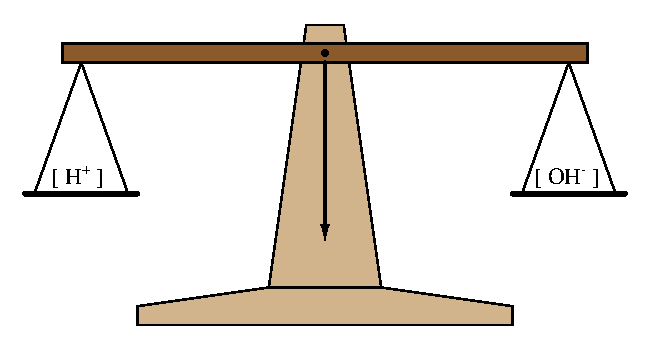
\includegraphics[width=15.5cm]{i00615x01.eps}$$

I rent vann er denne ``vekten'' balansert: [H$^{+}$] = [OH$^{-}$]. Tilsetting av syre tipper vekten den ene veien, base den andre.

Produktet av disse molaritetene er tilnærmet konstant for fortynnede vannløsninger ved fast temperatur. Dette er {\it ioniseringskonstanten for vann}, $K_W$:

$$K_W = [\hbox{H}^{+}] [\hbox{OH}^{-}] = 1.00 \times 10^{-14} \hbox{ at } 25^{o} \hbox{ C}$$

\vskip 10pt

\vskip 20pt

Anta at vi tilsetter syre til rent vann til [H$^{+}$] = 0.00027 $M$. Beregn pH ved 25$^{o}$ C.

\vskip 50pt

Anta at vi tilsetter base til rent vann til [OH$^{-}$] = 0.0081 $M$. Beregn pH ved 25$^{o}$ C.

\vskip 50pt

Som hovedregel: hvordan relaterer pH for sure løsninger, basiske løsninger og rent vann seg til hverandre? Oppgi numeriske områder.

\underbar{file i00615}
%(END_QUESTION)





%(BEGIN_ANSWER)

For første løsning: $- \log 0.00027$ = 3.57 pH

\vskip 10pt

For andre løsning: $- \log {1 \times 10^{-14} \over 0.0081}$ = $14 - (- \log 0.0081)$ = 11.91 pH

\vskip 10pt

Syrer har pH under 7, baser (alkaliske/kaustiske) har pH over 7, og rent vann har pH 7.0 (ved 25$^{o}$ C).

\vskip 10pt

I vektanalogien tilsvarer balanse ([H$^{+}$] = [OH$^{-}$]) en {\it nøytral} løsning. Dette betyr ikke nødvendigvis pH 7.0; med temperaturavhengig $K_W$ kan en nøytral løsning ha annen pH enn 7.

%(END_ANSWER)





%(BEGIN_NOTES)



%INDEX% Kjemi, pH: (vektanalogi)
%INDEX% Kjemi, pH: syre
%INDEX% Kjemi, pH: base (caustic, eller alkaline)
%INDEX% Kjemi, pH: molaritetsberegning

%(END_NOTES)

